\documentclass[12pt,a4paper,oneside]{scrartcl}

\usepackage[utf8]{inputenc}
\usepackage[T1]{fontenc}
\usepackage{lmodern}
\usepackage{tcolorbox}
\usepackage{microtype}
\usepackage{geometry}
\geometry{left=3cm,right=2.5cm,top=3cm,bottom=3cm}
\usepackage{setspace}
\onehalfspacing

\usepackage{amsmath,amssymb,amsthm,mathtools}
\usepackage{bm}
\usepackage{dsfont}
\usepackage{physics}
\usepackage{nicefrac}
\usepackage{enumitem}
\setlist[itemize]{topsep=0pt, itemsep=2pt}

\usepackage{tikz}
\usetikzlibrary{arrows.meta, positioning}
\usepackage{pgfplots}
\pgfplotsset{compat=1.17}
\usepackage{graphicx}
\usepackage{caption}
\usepackage{subcaption}
\usepackage{etoolbox}
\usepackage{xcolor}
\usepackage{float}
\usepackage{wrapfig}

\KOMAoptions{parskip=half}

\definecolor{indigo}{RGB}{75,0,130}

% Theorem
\newtheorem{lemma}{Lemma}[section]
\newtheorem{definition}{Definition}[section]
\newtheorem{theorem}{Theorem}[section]

\newenvironment{lemmabox}[1][]{
	\refstepcounter{lemma}
	\begin{tcolorbox}[colback=teal!5!white,
		colframe=teal!60!black,
		fonttitle=\bfseries,
		boxrule=0.8pt,
		arc=3pt,
		left=8pt,right=8pt,top=6pt,bottom=6pt,
		title={Lemma \thelemma\if\relax\detokenize{#1}\relax\else\ (#1)\fi}]
		}{
	\end{tcolorbox}
}

\newenvironment{definitionbox}[1][]{
\refstepcounter{definition}
\begin{tcolorbox}[colback=blue!5!white,
	colframe=blue!60!black,
	fonttitle=\bfseries,
	boxrule=0.8pt,
	arc=3pt,
	left=8pt,right=8pt,top=6pt,bottom=6pt,
	title={Definition \thedefinition\if\relax\detokenize{#1}\relax\else\ (#1)\fi}]
	}{
\end{tcolorbox}
}

\newenvironment{theorembox}[1][]{
\refstepcounter{theorem}
\begin{tcolorbox}[colback=indigo!5!white,
	colframe=indigo!70!black,
	fonttitle=\bfseries,
	boxrule=0.8pt,
	arc=3pt,
	left=8pt,right=8pt,top=6pt,bottom=6pt,
	title={Theorem \thetheorem\if\relax\detokenize{#1}\relax\else\ (#1)\fi}]
}{
\end{tcolorbox}
}

% Kopf- und Fußzeile
\usepackage{scrlayer-scrpage}
\clearpairofpagestyles
\ihead{Optimal Control}
\ohead{WS 2025/26}
\cfoot{\pagemark}
\pagestyle{scrheadings}
\setcounter{section}{-1}

\begin{document}
	
	% Titelseite
	\begin{titlepage}
		\centering
		\vspace*{3cm}
		{\Huge\bfseries Optimal Control}\par
		\vspace{1.5cm}
		{\Large Wintersemester 2025/26}\par
		\vspace{0.5cm}
		{\Large Dozent: Prof. Dr. Andrea Iannelli}\par
		\vfill
		{\today}
	\end{titlepage}
	
	\pagenumbering{roman}
	\tableofcontents
	\clearpage
	\pagenumbering{arabic}
	
	\section{Introduction}
	\[
	\dot{x} = f(t,x,u), \quad x(t_0)=x_0, \quad t \in [t_0,t_f]
	\]
	\[
	f : [t_0,t_f]\times\mathbb{R}^{n_x}\times\mathbb{R}^{n_u} \to \mathbb{R}^{n_x}
	\]
	\[
	x = \text{state}, \quad u = \text{input}
	\]
	
	Initial Value Problem (IVP)
	
	Given $x_0, u(\cdot)$ we can compute $x(\cdot)$ \\
	\hspace*{23.5mm}$\rotatebox[origin=c]{90}{$\Rsh$}$ functions of time $\rotatebox[origin=c]{270}{$\Lsh$}$
	
	When is this possible? It depends on $f$.
	
	
	\begin{lemmabox}[Sufficient conditions]
		Existence \& Uniqueness of solutions of ODEs.\\
		Assume that
		\begin{itemize}[]
			\item $f$ is piecewise continuous in $t$ and $u$
			\item $f$ is globally Lipschitz in $x$
			\[
			\exists\, k(t,u)\, \text{ s.t. } \|f(t,x_1,u)-f(t,x_2,u)\|\le k(t,u)\|x_1-x_2\|,\ \forall x_1,x_2 \in \mathbb{R}^{n_x}
			\]
		\end{itemize}
		Then $x(\cdot)$ exists for all $t$ and is unique.
	\end{lemmabox}
	
	\paragraph{Remarks}
	\begin{itemize}[noitemsep]
		\item Lipschitz continuous $\Rightarrow$ continuous, but not the converse
		\item $\sqrt{x}$ is continuous but not Lipschitz, $\dot x = \sqrt{x}$ does not have a unique solution
		\item Continously differentiable $(\mathcal{C}^1)$ $\Rightarrow$ locally Lipschitz continous $\forall x_1,x_2 \in \mathcal{X} \subset \mathbb{R}^{n_x}$
		\item Locally Lipschitz continuous x guarantees existence \& uniqueness for small enough times
	\end{itemize}
	
	In this course we will assume $f \in\mathcal{C}^1$ and implicitely assume that $t_f$ is chosen such that $x(\cdot)$ exists in $[t_0,t_f]$. \\\\
	We do not need to worry about existence \& uniqueness!
	
	\paragraph{Goal in Optimal Control:}
	Design $u$ such that
	\begin{enumerate}
		\item $u(t) \in \underset{\uparrow}{\mathcal{U}(t)}$, $x(t) \in \underset{\uparrow}{\mathcal{X}(t)} \quad \forall t \in [t_0,t_f], \quad \mathcal{X}\subseteq\mathbb{R}^{n_x}, \ \mathcal{U}\subseteq\mathbb{R}^{n_u}$\\
			sets defining constraints on $u \& x$ \\
			\hspace*{10mm}$\Rightarrow$ Admissible input/state trajectories
		\item
			The system behaves optimally according to
			\[
			\underset{\uparrow}{J}(u) = \int_{t_0}^{t_f} \underset{\uparrow}{l}(t,x(t),u(t))\,dt + \underset{\uparrow}{\varphi}(t_f,x(t_f))
			\]
			\hspace*{18mm}Cost function\hspace*{10mm}running cost\hspace*{10mm}terminal cost\\
			\hspace*{10mm}$\Rightarrow$ optimal behaviour
	\end{enumerate}
	
	Formally, we can state the goal as follows: \\
	Find an admissible input $u^\star$ which causes the dynamics to follow an admissible trajectory $x\star$ which minimizes $J$, that is
	\[
	\int_{t_0}^{t_f} l(t,x^\star(t),u^\star(t))\,dt + \varphi(t_f,x^\star(t_f)) \leq \int_{t_0}^{t_f} l(t,x(t),u(t))\,dt + \varphi(t_f,x(t_f))
	\]
	\hspace*{100mm}$\forall \text{ admissible } x,u$
	
	\paragraph{Examples of cost functions}
	\begin{enumerate}[label=\arabic*)]
		\item Minimum-time problem\\
		Goal: transfer the system from $x_0$ to a set $\mathcal{S}$ in the minimum time
		\[
		J = t_f-t_0 = \int_{t_0}^{t_f}dt \qquad (l=1, \varphi=0)
		\]
		\[
		x(t_f) \in \mathcal{S}
		\]
		Note: $t_f$ is also a decision variable! The unknowns are $(u,t_f)$.
		
		\item Minimum control-effort problem
		\[
		J = \int_{t_0}^{t_f} \|u(t)\|^2 \, dt
		\]
		\[
		x(t_f) \in \mathcal{S}
		\]
		
		\item Tracking problem
		\[
		J = \int_{t_0}^{t_f} (x(t)-r(t))^T Q (x(t)-r(t))dt
		\]
		$Q > 0$ (positive definit matrix: symmetric \& all eigenvalues positive) \\
		$r(t)$ given signal
	\end{enumerate}
	
	\section{Nonlinear Programming}
	
	Nonlinear Programs (NLP) are general \underline{finite-dimensional} optimization problems:
	\[
	\underset{x}{\min} f(x)
	\]
	\[
	\text{s.t. } g(x)\leq0, \quad h(x)=0
	\]
	$f: \mathbb{R}^n \to \mathbb{R}$, objective function\\
	$g: \mathbb{R}^n \to \mathbb{R}^{n_g}$, inequality constraints\\
	$h: \mathbb{R}^n \to \mathbb{R}^{n_h}$, equality constraints\\
	Feasible set:
	\[
	D = \{x\in\mathbb{R}^n \mid g(x)\leq0,\ h(x)=0\}
	\]
	$\bar{x}\in D$ feasible point
	
	\begin{definitionbox}[Global, local Minimizers]
			$x^\star\in \mathcal{D}$ \underline{Global Minimizer} of the NLP if
			\[
			f(x^\star)\le f(x)\quad \forall x\in \mathcal{D}
			\]
			$f(x^\star)$ is the \underline{Global Minimum} (or Minimum)\\
			Nomenclature: $x^\star$ is also called (optimal) solution, $F(x^\star)$ is optimal value\\
			$x^\star$ is a strict global minimizer if $f(x^\star)<f(x)\quad \forall x \in\mathcal{D}$\\
			$x^\star\in \mathcal{D}$ \underline{Local Minimizer} if
			\[
			\exists \varepsilon>0,\text{ s.t.}\ f(x^\star)\le f(x)\quad \forall x\in B_\varepsilon(x^\star)\cap \mathcal{D}
			\]
			\[
			B_\varepsilon(x) := \{ y \mid \|x-y\|\le\varepsilon\} \qquad \|\cdot\|:\mathbb{R}^n\to\mathbb{R}_{\geq 0}\text{ any norm in }\mathbb{R}^n
			\]
			Strict local Minimizer if inequality holds strictly\\
			Global min $\begin{tikzpicture}[baseline={(0,-0.25ex)}]
				% oberer Pfeil: nach rechts
				\draw[->] (0,0.2) -- (0.5,0.2);
				% unterer Pfeil: nach links
				\draw[<-] (0,0.0) -- (0.5,0.0);
				% Durchstreichung des unteren Pfeils
				\draw[line width=0.4pt] (0.1,-0.1) -- (0.4, 0.1);
			\end{tikzpicture}$ local min
	\end{definitionbox}
	
	Solving an NLP boils down to finding global or local minimizers. \\
	Does a solution always exist? No.
	
	
	
	
	\begin{definitionbox}[infimum]
		Given $\mathcal{S} \subseteq \mathbb{R}$, $\inf(\mathcal{S})$ is the greatest lower bound of $\mathcal{S}$:
		\begin{itemize}
			\item $z \geq \inf(\mathcal{S}), \quad \forall z \in \mathcal{S}\quad$ (lower bound)
			\item $\forall \bar{\alpha} > \inf(\mathcal{S}) \quad \exists z \in \mathcal{S}$ s. t. $ \bar{\alpha} > z\quad$ (greatest bound)
		\end{itemize}
	\end{definitionbox}
	
	\paragraph{Example}
		$\mathcal{S} = [-1,1], \, -50 = \inf(\mathcal{S})?\quad\to\quad$ No, $\inf(\mathcal{S}) = -1$	
	\begin{itemize}
		\item Analogous: $\sup(\mathcal{S})$ is smallest upper bound.  
		\item $\inf$ and $\sup$ always exist if $\mathcal{S} \neq \emptyset$
		\item $\inf(\mathcal{S})$ does not have to be an element of $\mathcal{S}$
		\item If $\mathcal{S}$ unbounded from below $\to$ $\inf(\mathcal{S})=-\infty$
		\item $\inf([a,b]) = \inf((a,b]) = a$
	\end{itemize}
	
	Connections with NLP?
	\[
	f: \mathcal{D} \to \mathbb{R}
	\]
	\[
	\inf(\underset{\mathcal{S}}{\underbrace{f(x)\,|\,x\in\mathcal{D}}}):=\bar{f}=\underset{x\in\mathcal{D}}{\inf}f(x) \quad\text{(similar to NLP)}
	\]
	
	Whenever NLP has solution, then NLP ist equivalent to this, but $\nexists x^\star \in \mathcal{D}$ s. t. $f(x^\star) = \bar{f}\quad\to\quad$ infimum exists, but not minimum
	
	\paragraph{Examples}
		$f(x) = e^{-x}, \quad \mathcal{D} = [0,\infty), \quad \inf(\mathcal{S}) = 0$ \\
		$f(x) = x, \quad \mathcal{D} =\mathbb{R}, \quad \inf(\mathcal{S}) = - \infty$, min doesn't exist! 
	\begin{figure}[H]
		\begin{center}
			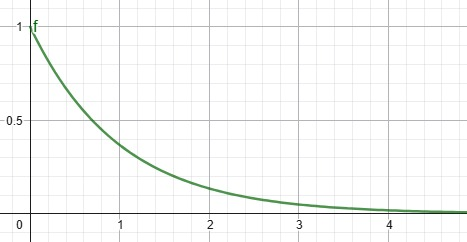
\includegraphics[width=0.4\textwidth]{images/1.0-1.jpg}
		\end{center}
	\end{figure}
		
	When does the infimum coincide with its optimal value?
	
	\begin{theorembox}[Extreme value problem) (Weierstrass Theorem]
		$f: D \to \mathbb{R},\,\mathcal{D} \subseteq \mathbb{R}^n$\\
		If:
		\begin{itemize}
			\item $f \in \mathcal{C}$ on $\mathcal{D}$
			\item $\mathcal{D}$ is compact
			\item $\mathcal{D} \neq \emptyset$
		\end{itemize}
		Then $f$ attains a minimum on $\mathcal{D}$.
	\end{theorembox}
	
	\begin{definitionbox}[Continuous function]
		$f: \mathcal{D} \to \mathbb{R}$ is continuous at $x\in\mathcal{D}$ if
		\[
			\forall \epsilon > 0 \exists \delta > 0 \text{ s. t. } \norm{x-x'} < \delta \quad \Rightarrow \quad \norm{f(x)-f(x')} < \epsilon
		\]
		If $f$ is continuous $\forall x \in \mathcal{D}$ then $f$ is continuous on $\mathcal{D}$ $\to$ $f \in \mathcal{C}$
	\end{definitionbox}
	
	Implication for NLP: If $f$ is $\mathcal{C}$ on $\mathcal{D}$ and $\mathcal{D}$ is compact and non-empty then [NLP] has a solution!
	
	\begin{itemize}
		\item $\mathcal{D} \subseteq \mathbb{R}^n$: in finite-dimensional spaces: compact = closed and bounded\\
		Not compact:
		\begin{itemize}
			\item $(a,b]\quad$ (not closed)
			\item $(-\infty,b]\quad$ (unbounded)
		\end{itemize}
		Compact set:
		\begin{itemize}
			\item $[a,b]\quad-\infty<a<b<\infty$
		\end{itemize}
	
	\paragraph{Warning:}
	$\mathcal{D}$ infinite dimensional (e.\,g. function space) then\\
	\hspace*{10mm}compact $\begin{tikzpicture}[baseline={(0,-0.25ex)}]
		% oberer Pfeil: nach rechts
		\draw[->] (0,0.2) -- (0.5,0.2);
		% unterer Pfeil: nach links
		\draw[<-] (0,0.0) -- (0.5,0.0);
		% Durchstreichung des unteren Pfeils
		\draw[line width=0.4pt] (0.1,-0.1) -- (0.4, 0.1);
	\end{tikzpicture}$ bounded and closed
	
	\begin{figure}[H]
		\centering
		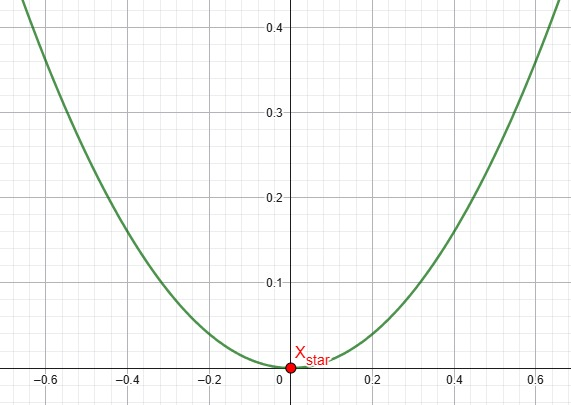
\includegraphics[width=0.4\textwidth]{images/1.0-2.jpg}
	\end{figure}	
	Theorem 1.1 is restrictive e.\,g. $f(x) = x^2, \mathcal{D} = (-\infty,\infty)$ has unique minimum
	\item Notation convention: Technically it is 'wrong' to write
	\[
		\min\underset{x\in\mathcal{D}}{f(x)}
	\]
	more compact is:
	\[
		\text{minimize}\,\underset{x\in\mathcal{D}}{f(x)} \quad \text{or} \quad \underset{x\in\mathcal{D}}{\inf}f(x)
	\]
	\end{itemize}
	
	Goal of the Chapter: characterize necessary and sufficient conditions for $x^\star$ to be global minimizer of NLP.
	
	\subsubsection*{Convexity}
	
	\begin{definitionbox}[Convex sets \& functions]
		\begin{itemize}
			\item A set $C \subseteq \mathbb{R}^n$ is \underline{convex} (cvx) if $\forall x, y \in C$
			\[
			\{ z \mid z = \lambda x + (1-\lambda)\lambda, \, \lambda \in [0,1]\}\subseteq C
			\]
			\begin{figure}[H]
				\begin{center}
					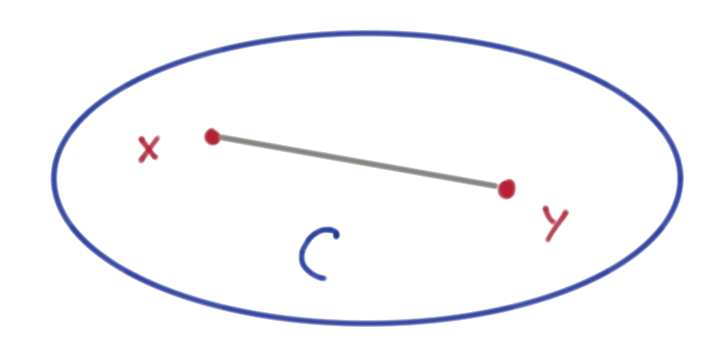
\includegraphics[width=0.23\textwidth]{images/1.0-3.png}
				\end{center}
			\end{figure}
			\item Given a cvx set $C$, a function $f: C \to \mathbb{R}$ is cvx if
			\[
			f(\lambda x + (1 - \lambda)y) \leq \lambda f(x) + (1 - \lambda) f(y), \quad\forall x,y \in C, \quad\lambda \in (0,1)
			\]
			\begin{figure}[H]
				\begin{center}
					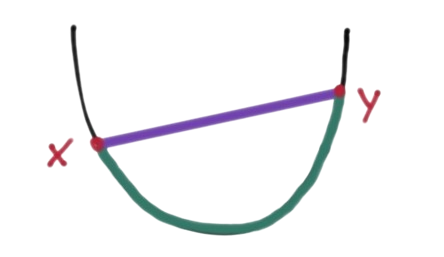
\includegraphics[width=0.3\textwidth]{images/1.0-4.png}
				\end{center}
			\end{figure}
			\item f is strictly cvx if the inequality holds strictly.
		\end{itemize}
		
	\end{definitionbox}
	
	\paragraph{Remarks}
	\begin{itemize}
		\item The definition extends to vector functions $f:C\to\mathbb{R}^n$ for convex $f_i$
		\item $f: C_1 \cross C_2 \to \mathbb{R}$\\
		$f(x,y)$ is jointly cvx, in $x,y$ if $z:=\begin{bmatrix}x\\y\end{bmatrix},\,f(z)$ is in cvx in $z$.
	\end{itemize}
		
	
	
	\paragraph{Example}
		$f(x,y) = x^2+y^2,\,z=\begin{bmatrix}x\\y\end{bmatrix}\to f(z) = z_1^2+z_2^2$
	
	\begin{definitionbox}
		An NLP is a \underline{convex program} if
		\begin{itemize}
			\item $f$ is convex function,
			\item $\mathcal{D}$ is convex set.
		\end{itemize}
	\end{definitionbox}
	
	\begin{lemmabox}
		Let $x^\star$ be a local minimizer of cvx program.  
		Then $x^\star$ is also global minimizer.
	\end{lemmabox}
	
	\textbf{Proof}: try as an erxercise\\
	
	Minimizers of convex NLP form a convex set.\\
	This set might be empty (Convex NLPs not guaranteed to have solution).\\
	\underline{However}: Unique solution for \underline{strictly} convex NLPs, if a solution exists.
	
	\begin{lemmabox}[First/Second order conditions for convexity]
		\begin{enumerate}
			\item $f:C\to\mathbb{R}$ continuously differentiable on $C$. Then $f$ is cvx iff
			\[
				f(y)\geq f(x)+\nabla f(x)^T(y-x), \quad\forall x,y\in C
			\]
			\[
				(\nabla f)_i = \frac{\partial f}{\partial x_i} \text{ is gradient (sometimes $f_{x_i}$)}
			\]
			\item $f$ twice differentiable on $C$, then $f$ convex iff
			\[
				\nabla_{xx}^2 f(x) \geq 0 \quad \forall x \in C
			\]
			\[
				(\nabla_{xx}^2)_{i,j} = \frac{\partial^2 f}{\partial x_i \partial x_j} \quad \text{(Hessian)}
			\]
		\end{enumerate}
	\end{lemmabox}
	
	\begin{itemize}
		\item $A\geq0$ means that: $A=A^T$ and pos semi-definite, i.\,e. all eigenvalues non-negative
		\item $f$ strictly cvx if $\nabla_{xx}^2 f(x) > 0 \quad \forall x \in C$ with $A>0$ meaning pos definite and symmetric
		\item Interpretation: Curvature of function should be non-negative/positive
		\item For exercises to check convexity, the second condition is generelly useful. First condition is useful for proofs.
	\end{itemize}
	
	For $\mathcal{D} = \{ x \mid g(x) \leq 0, \, h(x) = 0 \}$ the following holds: If
	
	\begin{minipage}{0.65\textwidth}
		\begin{itemize}
			\item $g$ are convex functions,
			\item $h$ are affine functions (i.e. $h(x) = 0 \Leftrightarrow Ax=b$),
		\end{itemize}
	\end{minipage}
	\begin{minipage}{0.15\textwidth}
		$\left.\vphantom{\begin{array}{l}g\\h\end{array}}\right\}$ sufficient
	\end{minipage}
	
	
	then $\mathcal{D}$ is a convex set.
	
	\paragraph{Example} $a,b\in\mathbb{R}$
	
	\begin{table}[H]
		\centering
		\begin{tabular}{c c c}
			$\underset{x}{\min}f$ & & $\underset{x}{\min}f$\\
			s.t. $x^3-1\leq0$ & $\qquad\leftrightarrow\qquad$ & s.t. $x-1\leq0$\\
			$(ax+b)^2=0$ & & $ax+b=0$\\
			non-convex & & convex\\
			non-affine & & affine
		\end{tabular}
	\end{table}
	
	\underline{Moral to recognize convexity of NLP:}
	\begin{enumerate}
		\item Use definition of cvx NLP, cvx $f$, convex $\mathcal{D}$
		\item If $\mathcal{D}$ written as equality/inequality-constraints, check $g$ convex/$h$ affine.\\
		If not, check further whether the feasible set is cvx or not (e.g. can be written equivalently with cvx $g$/affine $h$).
	\end{enumerate}
	
	\subsection{Unconstrained Problems}
	\[
		\mathcal{D} = \mathbb{R}^n
	\]
	Assume throughout that $f \in \mathcal{C}^1$ (continuously differentiable).
	
	\begin{definitionbox}[Descent Direction]
		$d \in \mathbb{R}^n$ is a \underline{descent direction} for $f$ at $\bar{x} \in \mathbb{R}^n$ if
		\[
		\exists \delta > 0 \quad \text{s.t.} \quad f(\bar{x} + \lambda d) < f(\bar{x}) \quad \forall \lambda \in (0, \delta).
		\]
		$F(\bar{x})$: \underline{Cone of decent directions}\\
		Set of all descent directions of $f$ at $\bar{x}$
	\end{definitionbox}
	
	A set $K \subseteq \mathbb{R}^n$ is a cone if it contains the full ray through any point in the set.
	
	\[
		K \text{ cone if }\forall x\in K \text{ and } \rho \geq 0, \quad \rho x \in K
	\]
	
	\begin{figure}[H]
		\begin{center}
			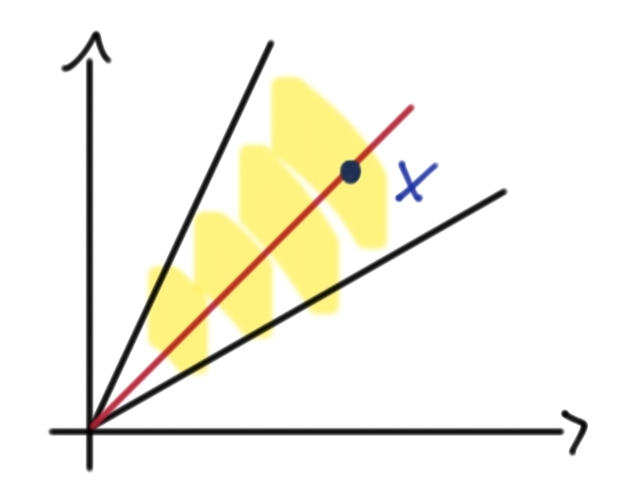
\includegraphics[width=0.4\textwidth]{images/1.1-1.jpg}
		\end{center}
	\end{figure}
	
	This is a geometric characterization of descent direction. It gives us a geometric condition for $x^\star$ to be a local minimizer.
	
	\begin{lemmabox}[Geometric Condition for local minimum]
		$x^\star$ is a local minimizer iff
		\[
		\mathcal{F}(\bar{x}) = \emptyset.
		\]
	\end{lemmabox}
	
	We want an algebraic condition to be able to compute or look for $x^\star$.
	
	\begin{lemmabox}[Algebraic first-order characterization of $\mathcal{F}$]
		If $\nabla f(\bar{x}) \neq 0$, then
		\[
		\mathcal{F}_0(\bar{x}) = \{ d \mid \nabla f(\bar{x})^T d < 0 \} = \mathcal{\mathcal{F}}(\bar{x}).
		\]
		Otherwise
		\[
		\mathcal{F}_0(\bar{x}) \subseteq \mathcal{F}(\bar{x}).
		\]
	\end{lemmabox}
	
	\textbf{Proof}: try Taylor-series expansion of $f$ at $\bar{x}$
	
	Graphical interpretation:
	
	
	
	$\nabla f$ forms angles greater or equal than $90^\circ$ with \underline{all} descent directions.
	
	\begin{lemmabox}[First-order necessary condition for local minimum]
		If $x^\star$ is a local minimizer, then
		\[
		\underset{\text{'stationary point'}}{\underbrace{\nabla f(x^\star) = 0}}.
		\]
	\end{lemmabox}
	
	\textbf{Proof}: Contradiction\\
	If $\nabla f(x^\star) \neq 0$, then $d = -\nabla f(x^*) \neq 0$. Therefore there exists a descent direction $d\in\mathcal{F}(x^\star)$ by Lemma 1.4. Thus $\exists \delta > 0$ s.t. $f(x^\star+\lambda d)<f(x^\star) \quad \forall\lambda\in (0,\delta).$\\
	This is a contradiction with the fact, that $x^\star$ is a minimizer.\hfill\qedsymbol{}
	
	Why only necessary?\\
	It can't be a sufficient condition because in case where $\nabla f(x^\star) = 0$ we cannot use Lemma 1.4, e.g. $f_1(x) = -x^2,\,f_2(x) = x^3,\,\nabla f_1(0) = \nabla f_2(0) = 0.$
	
	\begin{lemmabox}[second order necessary condition]
		Assume f is twice continuously differentiable $f \in \mathcal{C}^2$
		\[
			x^\star\text{ local minimizer }\Rightarrow \nabla_{xx}^2 f(x^\star) \geq 0
		\]
	\end{lemmabox}
	
	\textbf{Note:} the condition on the Hessian of f can be interpreted as a local convexity property (around $x^\star)$.
	
	\textbf{Proof:} $2^{nd}$ order Taylor expansion around $x^\star$ in direction $d \in \mathbb{R}^n$:
	\[
		f(x^\star + \lambda d) = f(x^\star) + \lambda\nabla f(x^\star)^Td + \frac{\lambda^2}{2}d^T \nabla_{xx}^2 f(x^\star) d + \lambda^2\norm{d}^2\alpha (\lambda d)
	\]
	\[
		(\to\alpha(\cdot)) \text{ is a function that is order $1$ or higher in $\lambda d$})
	\]
	\begin{enumerate}
		\item If $x^\star$ is local minimzer $\Rightarrow\nabla f(x^\star) = 0$
		\item Divide by $\lambda^2$:
		\[
			\frac{f(x^\star+\lambda d)-f(x^\star)}{\lambda^2} = \frac{1}{2} d^T \nabla_{xx}^2 f(x^\star) d + \norm{d}\alpha (\lambda d)
		\]
		\item $\lambda \to 0$ on the right-hand-side the first term dominates
		\[
			\frac{f(x^\star+\lambda d)-f(x^\star)}{\lambda^2} \approx \frac{1}{2} d^T \nabla_{xx}^2 f(x^\star) d
		\]
		\item For $x^\star$ is a local minimizer, the left-hand-side must be $\geq 0$ for any $d\in\mathbb{R}^n$\\$\hspace*{1cm}\Rightarrow\quad d^T \nabla_{xx}^2 f(x^\star) \geq 0 \quad\forall d\quad \Rightarrow\quad \nabla_{xx}^2 f(x^\star)\geq0$\hfill\qedsymbol{}
	\end{enumerate}
	
	Only a necessary condition, because when $\nabla_{xx}^2 f(x^\star)$ is singular, we need to use higher-order information.
	
	Generally it is hard to get (global) sufficient conditions. $\to$ convexity to the rescue!
	
	\begin{lemmabox}[First order N\&S condition for global minimizers]
		Assume f is convex.
		\[
			\exists x^\star \text{ s.t. } \nabla f(x^\star) = 0 \quad\Leftrightarrow\quad x^\star \text{ is a global minimizer}
		\]
		If $f$ is  strictly convex, then the minimizer is unique.
	\end{lemmabox} 	
	
	\textbf{Proof}: $(\nabla f = 0\,\Rightarrow\,\text{global minimum})$
	
	First order condition for convexity:
	\[
		f(y) \geq f(x) + \nabla f(x)^T(y-x),\quad\forall x,y\in\mathbb{R}^n
	\]
	Pick $x = x^\star$:
	\[
		f(y) \geq f(x^\star),\quad\forall y\in\mathbb{R}^n
	\]
	(Other direction holds because of Lemma 1.5)
	
	What if we do not have global convexity?
	
	\begin{lemmabox}[Second order sufficient condition for local minimizer]
		Assume $f \in\mathcal{C}^2$.\\
		If $\nabla f(x^\star) = 0$ and $\nabla_{xx}^2 f(x^\star) > 0\quad\Rightarrow\quad x^\star$ is strict local minimizer.
	\end{lemmabox}
	
	\textbf{Proof}: Taylor expansion (Similar to Lemma 1.6)
	
	\subsection{Constrained optimization}
	
	\[
		\mathcal{D} \subseteq\mathbb{R}^n,\quad\mathcal{D} = \{x \mid g_i(x)\leq0,\,i=1,\dots,n_g\quad h_j(x)=0,\,j=1,\dots,n_h\}
	\]
	
	We assume throughout $g_i,\,h_j$ are all $\mathcal{C}^1$ functions.
	
	\begin{definitionbox}[Tangent vector, tangent cone]
		$p\in\mathbb{R}^n$ is a tangent vector to $\mathcal{D}$ at $\bar{x}\in\mathcal{D}$ if $\exists$ differential curve $\bar{x}(s):[0,\epsilon)\to\mathcal{D}$ with $\epsilon>0$ such that $\bar{x}(0)=\bar{x},\left.\frac{d\bar{x}}{ds}\right|_{s=0}=p$.\\\\
		Tangent cone $\mathcal{T}_\mathcal{D}(\bar{x})$ to $\bar{x}$ is the set of all tangent vectors
		\[
			\mathcal{T}_\mathcal{D}(\bar{x}):=\{p\mid p \text{ tangent vector to $\mathcal{D}$ at $\bar{x}$}\}
		\]
	\end{definitionbox}
	
	Graphical representation:
	
	Set of directions that make us stay feasible (at least infinitesimally)
	
	When it comes to geometric conditions for optimality in constrained problems, we now have 2 sets/2 directions:
	\begin{itemize}
		\item $d\in\mathcal{F}(x)\to$ descent direction: objective improves
		\item $d\in\mathcal{T}_D(\bar{x})\to$ tangent vector: we stay feasible
	\end{itemize}
	
	\begin{lemmabox}[Geometric condition for local minimizer, $\mathcal{D}\subseteq\mathbb{R}^n$]
		$x^\star$ is a local minimizer iff $\mathcal{F}(\bar{x})\cap\mathcal{T}_\mathcal{D}(\bar{x})=\emptyset$
	\end{lemmabox}
	
	It is basically says that 'any improving direction can't be feasible'.
	
	
	
	As in the unconstrained case, we want to turn geometric conditions to algebraic ones.
	
	\begin{lemmabox}[$1$st order Nec. condition - semi-algebraic]
		If $x^\star$ is a local minimizer. Then:
		\begin{enumerate}
			\item $x^\star\in\mathcal{D}$
			\item $\underset{\text{geometric}}{\underline{\forall p\in\mathcal{T}_\mathcal{D}(x^\star)}}$, it holds $\underset{\text{algebraic}}{\underline{p^T\nabla f(x^\star)\geq 0}}$
		\end{enumerate}
	\end{lemmabox}
	
	\textbf{Proof}:
	
	Item 1 $\to$ feasibility
	
	Item 2: Assume there is a $p$ s.t. $p^T\nabla f(x^\star)<0$. Then 
	\[
		\exists\text{ curve }\bar{x}(s)\in\mathcal{D}\text{ s.t. }\left.\frac{df(\bar{x})}{ds}\right|_{s=0} \underset{\rotatebox[origin=c]{90}{$\Rsh$}\text{ chain rule }}{=p^T\nabla f(x^\star})<0
	\]
	which would mean that $p$ is descent direction. Contradicts $x^\star$ local minimizer.
	
	This is almost a translation of Lemma 1.9 because we replaced $\mathcal{F}(x^\star)$ with its \underline{algebraic} form '$d^T\nabla f(x^\star)<0'$.
	
	To obtain a fully algebraic test, we need a few more concepts.
	
	\begin{definitionbox}[Active constraints, active set, regular points]
		$\bar{x}\in\mathcal{D}$
		\begin{itemize}
			\item $g_i$ is \underline{active} at $\bar{x}$ if $g_i(\bar{x})=0$
			\item $A(\bar{x}) = \{i\mid g_i(\bar{x})=0\}$ \underline{set of active constraints} at $\bar{x}$
			\item $\bar{x}\in\mathcal{D}$ is a \underline{regular point} if $\nabla g_i(\bar{x}),\,i\in\mathcal{A}(\bar{x})$ and $\nabla h_j(\bar{x}),\,j=1,\dots,n_h$ are linearly independent.
		\end{itemize}
	\end{definitionbox}
	
	\begin{lemmabox}[Algebraic first-order characterization of target set]
		If $\bar{x}$ is regular point. Then
		\[
			\mathcal{T}_\mathcal{D}(\bar{x})=\{p\mid\nabla h(\bar{x})^p=0,\,\nabla g_i(\bar{x})^p\leq0,\quad\forall i\in\mathcal{A}(\bar{x})\}\qquad\textcircled{1}
		\]
		where $\nabla h(\bar{x}):=[\nabla h_1(\bar{x}),\dots,\nabla h_{n_k}(\bar{x})]\in\mathbb{R}^{n\cross n_h}$.
		
		\textcircled{1} can be written equivalently as $\mathcal{T}_\mathcal{D}(\bar{x})=\{p\mid\mathcal{A}(\bar{x})p\geq0\}$
	\end{lemmabox}
	
	\[
	A(\bar{x}):=\left[
	\begin{array}{c}
		\nabla h(\bar{x})^T \\[4pt]
		-\nabla h(\bar{x})^T \\[4pt]
		\vdots \\[4pt]
		-\nabla g_i(\bar{x})^T \\[4pt]
		\vdots
	\end{array}
	\right]
	\begin{array}{l}
		\in\mathbb{R}^{(2n_h+\abs{\mathcal{A}(\bar{x})})\cross n} \\[6pt]
		\left.\rule{0pt}{3.0em}\right\} i\in\mathcal{A}(\bar{x})
	\end{array}
	\]
	
	In other words, item 2 of Lemma 1.10 can be written as follows:
	\[
		p\in\mathbb{R}^n:\, \mathcal{A}(x^\star)p\geq0,\,p^T\nabla f(x^\star)<0
	\]
	still not very tractable?
	
	Farkas Lemma to the rescue:
	
	\begin{lemmabox}[Farkas Lemma]
		For any matrix $A\in\mathbb{R}^{m\cross n}$, vector $b\in\mathbb{R}^n$.
		
		Exactly one of the following holds:
		\begin{enumerate}
			\item $\exists y\in\mathbb{R}^m\,y\geq0$, such that $A^Ty=b$
			\item $\exists p\in\mathbb{R}^m$, such that $A^Tp\geq0,\,p^Tb<0$
		\end{enumerate}
	\end{lemmabox}
	
	Take $A\equiv A(x^\star)$ and $b\equiv\nabla f(x^\star)$
	
	If we find $y$ satisfying 1., then 2. can't hold $\Rightarrow$ item 2 of Lemma 1.10 is verified $\Rightarrow$ $x^\star\in\mathcal{D}$ is a local minimizer.
	
	KTK-conditions just follow from imposing
	
	\hspace*{1cm}item 1 of Lemma 1.10 $\to$ $x^\star\in\mathcal{D}$
	
	\hspace*{1cm}item 2 of Lemma 1.10 $\to$ $\exists y\in\mathbb{R}^m,\,y\geq0$ s.t. $\mathcal{A}(x^\star)^Ty=\nabla f(x^\star)$
	
	\underline{\textbf{Conceptual summary}}\nopagebreak
	
	\begin{tikzpicture}[
		node distance=2.5cm and 5cm,
		box/.style={draw, rectangle, rounded corners, align=center, minimum width=4cm, minimum height=1.2cm},
		arrow/.style={-{Latex[length=3mm]}, thick}
		]
		
		% Nodes
		\node[box] (lemma19) {Lemma 1.9\\ \textit{exact geometric}\\ \textit{characterization of $x^\star$}};
		\node[box, right=of lemma19] (lemma110) {Lemma 1.10\\ \textit{semi-algebraic}\\ \textit{ necessary condition}};
		\node[box, below=of lemma110] (kkt) {KKT conditions\\ \textit{(1$^{st}$ order necessary conditions)}};
		
		% Arrows
		\draw[arrow] (lemma19) -- node[above, sloped, align=center] {algebraic expression\\ for $\mathcal{F}(x^\star)$} (lemma110);
		\draw[arrow] (lemma110) -- node[left, align=left]{- algebraic expression of $\mathcal{T}_\mathcal{D}(x^\star)$\\ - Farkas Lemma} (kkt);
	\end{tikzpicture}
\end{document}
